\section{Background}

% \subsection{Kubernetes}
% Kubernetes, commonly known as K8s, is an open-source platform that automates the deployment, scaling, and management of containerized applications. Developed from Google's extensive experience with running large-scale workloads, Kubernetes was released in 2014 and has quickly become the leading standard for managing container environments. It provides a robust framework for maintaining distributed systems, handling scaling and failover for applications, implementing various deployment strategies. Key features of Kubernetes include container orchestration, which automatically places containers based on resource needs and constraints; service discovery and load balancing, offering stable exposure and distribution of high-traffic container loads; and storage orchestration, which supports a variety of storage systems from local to cloud-based options like Google Cloud, Azure, and AWS. Furthermore, Kubernetes facilitates automated rollouts and rollbacks, allowing for controlled updates and maintaining system stability. It also offers automatic bin packing, optimizing resource utilization without sacrificing availability, and features self-healing capabilities, automatically managing container health by restarting or replacing containers as needed. This makes Kubernetes a highly versatile tool, useful in a wide range of settings from small startups to large enterprises, and supported by a vibrant community of developers and contributors.

% \subsection{diversity workload challenges}
% Microservices, AI, and big data workloads, while distinct in their demands and architectures, all benefit significantly from Kubernetes' versatile orchestration capabilities. Microservices are characterized by their small, independent, and dynamic nature, where each service performs a specific function and communicates using APIs. Kubernetes enhances microservices by providing excellent service discovery, load balancing, and the ability to perform rolling updates and rollbacks, which minimizes downtime during frequent updates. These features allow for independent scaling and updating of services without affecting the entire application ecosystem, making Kubernetes ideal for microservice management.

% AI workloads, in contrast, are computationally intensive and often require specialized hardware like GPUs. They deal with large data volumes and involve complex calculations, primarily during the training phase of machine learning models. Kubernetes caters to these needs through efficient resource allocation, including GPU management, and supports batch job scheduling to handle intensive, non-interactive tasks. This capability allows for the dynamic allocation and scaling of resources as computational demands fluctuate, which is crucial for optimizing AI operations.

% Big data workloads handle vast amounts of varied data, necessitating robust storage and powerful processing capabilities for both batch and real-time processing. Kubernetes supports these requirements with features like Persistent Volumes for reliable data storage across pod and node restarts, and StatefulSets for running databases and other applications that require persistent storage and unique network identifiers. This setup is vital for managing the volume, velocity, and variety of data characteristic of big data applications.

% Despite their differences, all these workloads share the need for high availability, resource efficiency, and scalability, which Kubernetes addresses with its core functionalities. Each workload leverages these features in unique ways—microservices focus on dynamic scalability and deployment, AI on resource-intensive computations, and big data on volume handling and processing efficiency. Kubernetes' ability to finely tune configurations and resource allocations makes it a powerful tool for managing the diverse and demanding environments typical of modern computing landscapes

Despite the advanced optimization features of Kubernetes, a significant challenge remains in the discrepancy between resource allocation and utilization. This gap arises from the disparity between client demands, typically driven by estimate peak usage, and the long-term resource requirements of certain services. As clients lack full control over user behavior over time, the utilization of allocated resources fluctuate over the life span of the application across a period of time, this example is illustrated in Fig. \ref{fig:day_use}. Use the web server as an example that demonstrates the characteristic that the requests from users may peak at noon and gradually fall in the evening. In the night time, low utilization of the requested resources contribute the majority of waste. 

In the context of this project, the terms "colocation" and "over-commitment" are often used interchangeably; however, they actually refer to distinct concepts. Colocation specifically refers to scheduling different workloads within a single container. Over-commitment, on the other hand, involves assigning workloads to clusters such that the total sum of requested resources exceeds the total allocatable resources at typical.

\begin{figure*}[h]
    \centering
    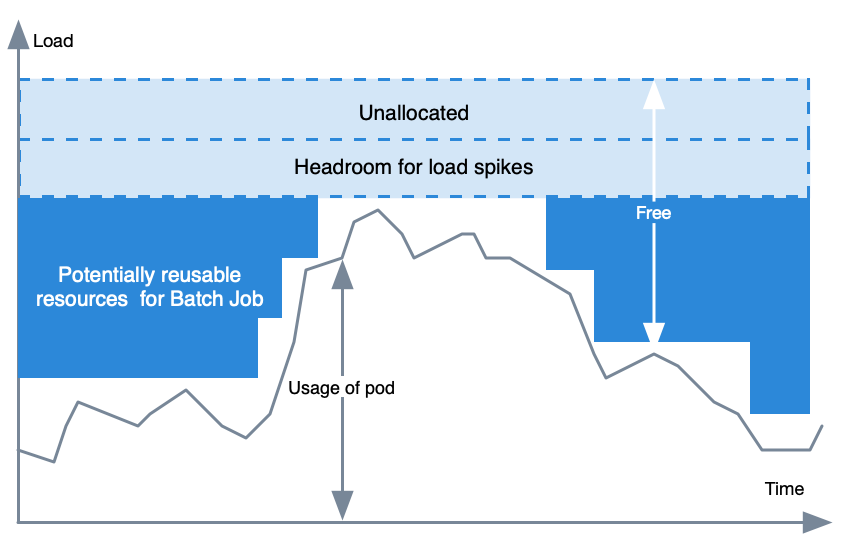
\includegraphics[width=0.6\textwidth]{img-load-explain.png}
    \caption{Illustration of the fluctuated request resource utilization over period of time}
    \label{fig:day_use}
\end{figure*}